\documentclass[11pt, a4paper, twocolumn]{article}
\usepackage[utf8]{inputenc}
\usepackage[spanish]{babel}
\usepackage{graphicx}
\usepackage{fancyhdr}
\usepackage{geometry}
\usepackage{amsmath, amssymb, amsfonts}
\usepackage{booktabs}
\usepackage{multirow}
\usepackage{enumitem}
\usepackage{xcolor}
\usepackage{hyperref}
\usepackage{natbib}
\usepackage{url}
\usepackage{tikz}
\usepackage{float}
\usepackage{microtype}
\usepackage{amsmath, amssymb}
\usepackage[numbers]{natbib}  % Para citas tipo [1], [2]
\usepackage{hyperref}
\usepackage{breakurl} % Opcional si usas pdflatex
\usepackage{url}
\usepackage{hyperref}
\usepackage{abstract}
\usepackage{booktabs}
\usepackage{tabularx}
\usepackage{makecell}


\usepackage{float}
\usepackage{caption}
\setlength{\columnsep}{1cm}
\geometry{margin=2.5cm, headheight=15pt, headsep=1.4cm}
\renewcommand{\abstractname}{}           % elimina el título "Resumen" / "Abstract"
\renewcommand{\absnamepos}{empty}

\renewenvironment{abstract}{
  \small\itshape
}{\par}

%\definecolor{maincolor}{RGB}{0, 83, 134}
%\definecolor{secondcolor}{RGB}{0, 124, 180}

\hypersetup{
    colorlinks=true,
    linkcolor=black,
    filecolor=black,
    urlcolor=black,
    citecolor=black,
    pdftitle={Optimización de la Planificación de Capacidad Aeroportuaria en el Perú Usando Métodos de Punto Interior},
    pdfauthor={Belinda Apaza Quispe},
    pdfsubject={Métodos de Optimización},
    pdfkeywords={optimización, programación lineal, puntos interiores, logística aérea}
}

\pagestyle{fancy}
\fancyhf{} 

\fancyhead[L]{
\includegraphics[height=1cm]{unap.png}}
\fancyhead[C]{%
\begin{tabular}{c}
\textbf{Universidad Nacional del Altiplano} \\ 
{\small Facultad de Ingeniería Estadística e Informática}
\end{tabular}}
\fancyhead[R]{
\includegraphics[height=1cm]{FINESI.png}}

\fancyfoot[L]{\small \textit{Métodos de Optimización}} 
\fancyfoot[C]{\small \thepage} 
\fancyfoot[R]{\small \textit{\today}} 



\title{\textbf{Optimización de la Planificación de Capacidad Aeroportuaria en el Perú Usando Métodos de Punto Interior}}
\author{Belinda Apaza Quispe\\
{\small Facultad de Ingeniería Estadística e Informática} \\
{\small Universidad Nacional del Altiplano – Puno} \\
{\small Puno, Perú}}
\date{}

\begin{document}


\maketitle

\begin{abstract}
\selectlanguage{english}
\textbf{Abstract - This study presents an application of Interior Point Methods to solve an optimization problem in the context of airport traffic in Peru, using OSITRAN data collected from 2019 to 2025. The objective is to assign optimal capacities to airports, month by month, in a way that minimizes the difference between actual passenger demand and the assigned capacity, under a budget constraint. Using a convex optimization model implemented in Python with the CVXPY library, we obtained an efficient capacity allocation for various time periods, achieving a close match between observed demand and optimized capacity. The results are presented through comparative graphs that demonstrate the effectiveness of the proposed approach.}

\textbf{Keywords: convex optimization, interior‑point methods, Peru.}
\selectlanguage{spanish}
\end{abstract}

\setcounter{secnumdepth}{0}

\renewenvironment{abstract}{
  \small
  \begin{center}\bfseries\abstractname\end{center}%
  \itshape
}{
  \par
}

\section{Introducción}

En los últimos años, la gestión eficiente del tráfico aeroportuario se ha convertido en un elemento crítico para el desarrollo económico y la conectividad regional del Perú. El aumento sostenido del flujo de pasajeros, especialmente en aeropuertos concesionados como los gestados por Aeropuertos del Perú (ADP) y Aeropuertos Andinos del Perú (AAP), exige el uso de técnicas de optimización avanzadas que asignen recursos operativos de manera eficiente y ajustada a la demanda real \citep{centreforaviation_peru}.

Este estudio utiliza los Métodos de Punto Interior —también conocidos como interior-point methods— una familia de algoritmos de complejidad polinómica introducida por Karmarkar en 1984, cuya eficiencia en problemas grandes y convexos es comparable e incluso superior al del método simplex \citep{karmarkar1984,newtonipm}. Estos algoritmos recorren el interior de la región factible, otorgando robustez en entornos con múltiples restricciones operativas.

Los datos utilizados provienen de OSITRAN (Organismo Supervisor de la Inversión en Infraestructura de Transporte de Uso Público), que proporciona información oficial mensual de tráfico de pasajeros en aeropuertos concesionados desde enero de 2019 hasta marzo de 2025. Según sus reportes, las inversiones acumuladas en infraestructura aeroportuaria superaron los USD 588 millones a comienzos de 2023, distribuidos entre LAP, ADP y AAP \citep{ositran2023inversion}.

El principal objetivo es asignar óptimamente la capacidad mensual al tráfico aeroportuario, minimizando la brecha entre la demanda real y la capacidad asignada, dentro del marco de un presupuesto acotado. Este enfoque requiere un modelo de programación convexa altamente escalable.

Finalmente, la capacidad asignada se compara con la demanda real registrada por OSITRAN, lo que permite identificar aeropuertos con subutilización o saturación, apoyando la toma de decisiones estratégicas a nivel nacional.

\section{Metodologia y materiales}

\subsection{Optimización Convexa}
La optimización convexa trata problemas con función objetivo convexa y restricciones convexas o afines, lo que garantiza que cualquier mínimo local sea global \citep{convex_global_minimum}. Esto es esencial en aplicaciones como la gestión aeroportuaria, donde se requiere estabilidad y precisión en la asignación de recursos bajo demanda variable.


\subsection{Métodos de Punto Interior}
Los métodos de punto interior fueron introducidos en 1984 por Karmarkar, marcando un hito en la resolución polinómica de problemas convexos :contentReference. Los enfoques más utilizados son: \\
\\
\textbf{Método de barrera}: incorpora una penalización logarítmica para mantener la iteración dentro del dominio factible. \\
\textbf{Método primal-dual}: El método primal‑dual se basa en las condiciones de Karush–Kuhn–Tucker (KKT) para asegurar óptimos con restricciones \citep{KKT_wiki}.


Estos métodos convergen superlinealmente y suelen requerir un número reducido de iteraciones, independientemente de la escala del problema :\citep{cvxpy_solvers}

\textbf{CVXPY} es un lenguaje de modelado en Python que permite definir problemas convexos con sintaxis intuitiva. Internamente, traduce el problema a formas estándar y delega la resolución a solvers como CVXOPT, que emplea algoritmos de punto interior \citep{cvxopt_coneprog}. CVXOPT ofrece opciones como \texttt{max\_iters}, \texttt{abstol}, \texttt{feastol}, y distintos métodos para resolver los sistemas KKT.

\subsection{Aplicaciones al Tráfico Aeroportuario}
La planificación de capacidad aeroportuaria se presta naturalmente a una formulación convexa. Por ejemplo, en \emph{Second‑Order Cone Programming} (SOCP) se modelan restricciones de capacidad y flujo mediante normas euclidianas, resolubles con métodos de punto interior : 
Además, en el ámbito del control de tráfico aéreo, Work y Bayen (2008) presentaron modelos que minimizan demoras usando programas lineales o cuadráticos . Otro punto clave: se garantiza que el óptimo encontrado es global, gracias a la convexidad del problema.

\subsection{Datos}

El conjunto de datos utilizado proviene del \textit{Portal de Datos Abiertos del Gobierno del Perú}, específicamente del registro mensual de tráfico de pasajeros por tipo de vuelo en aeropuertos concesionados por las entidades ADP y AAP. El periodo considerado abarca desde enero de 2019 hasta marzo de 2025. Las variables principales consideradas en este estudio incluyen: nombre del aeropuerto, mes, año, tipo de vuelo y total de pasajeros transportados.

Para reducir la complejidad del problema y facilitar la visualización de los resultados, se seleccionaron tres aeropuertos y un subconjunto de meses representativos. Los datos fueron agregados por aeropuerto, año y mes para calcular la demanda mensual de pasajeros.

El conjunto completo puede consultarse en el portal de datos abiertos del OSITRAN:

\footnotesize
\noindent Fuente de datos: \href{https://datosabiertos.gob.pe/dataset/informacion-trafico-de-pasajeros-por-tipo-de-vuelo-adp-aap-ene-2019-mar-2025-organismo}{Portal de Datos Abiertos del Gobierno del Perú – OSITRAN}


\subsubsection*{Estadísticas Descriptivas}

A continuación se presentan algunas estadísticas descriptivas del total de pasajeros por aeropuerto y tipo de vuelo para el período 2019–2025:

\begin{table}[H]
\centering
\caption{Estadísticas descriptivas del total de pasajeros por registro}
\label{tab:estadisticas_descriptivas}
\begin{tabular}{lr}
\toprule
\textbf{Estadístico} & \textbf{Valor} \\
\midrule
Cantidad de registros & 2,741 \\
Media & 19,843.13 \\
Desviación estándar & 34,336.63 \\
Mínimo & 0 \\
Percentil 25 & 0 \\
Mediana (50\%) & 92 \\
Percentil 75 & 30,947 \\
Máximo & 224,479 \\
\bottomrule
\end{tabular}
\end{table}

Hay mucha dispersión: algunos aeropuertos tienen tráfico muy bajo (0–100 pasajeros), mientras otros superan los 200,000 pasajeros al mes. \\

El $25\%$ de los registros son cero: hay muchos aeropuertos sin vuelos en varios meses.\\

La media está muy por encima de la mediana, lo cual indica asimetría positiva (unos pocos aeropuertos concentran gran parte del tráfico).\\

\begin{figure}[H]
\centering
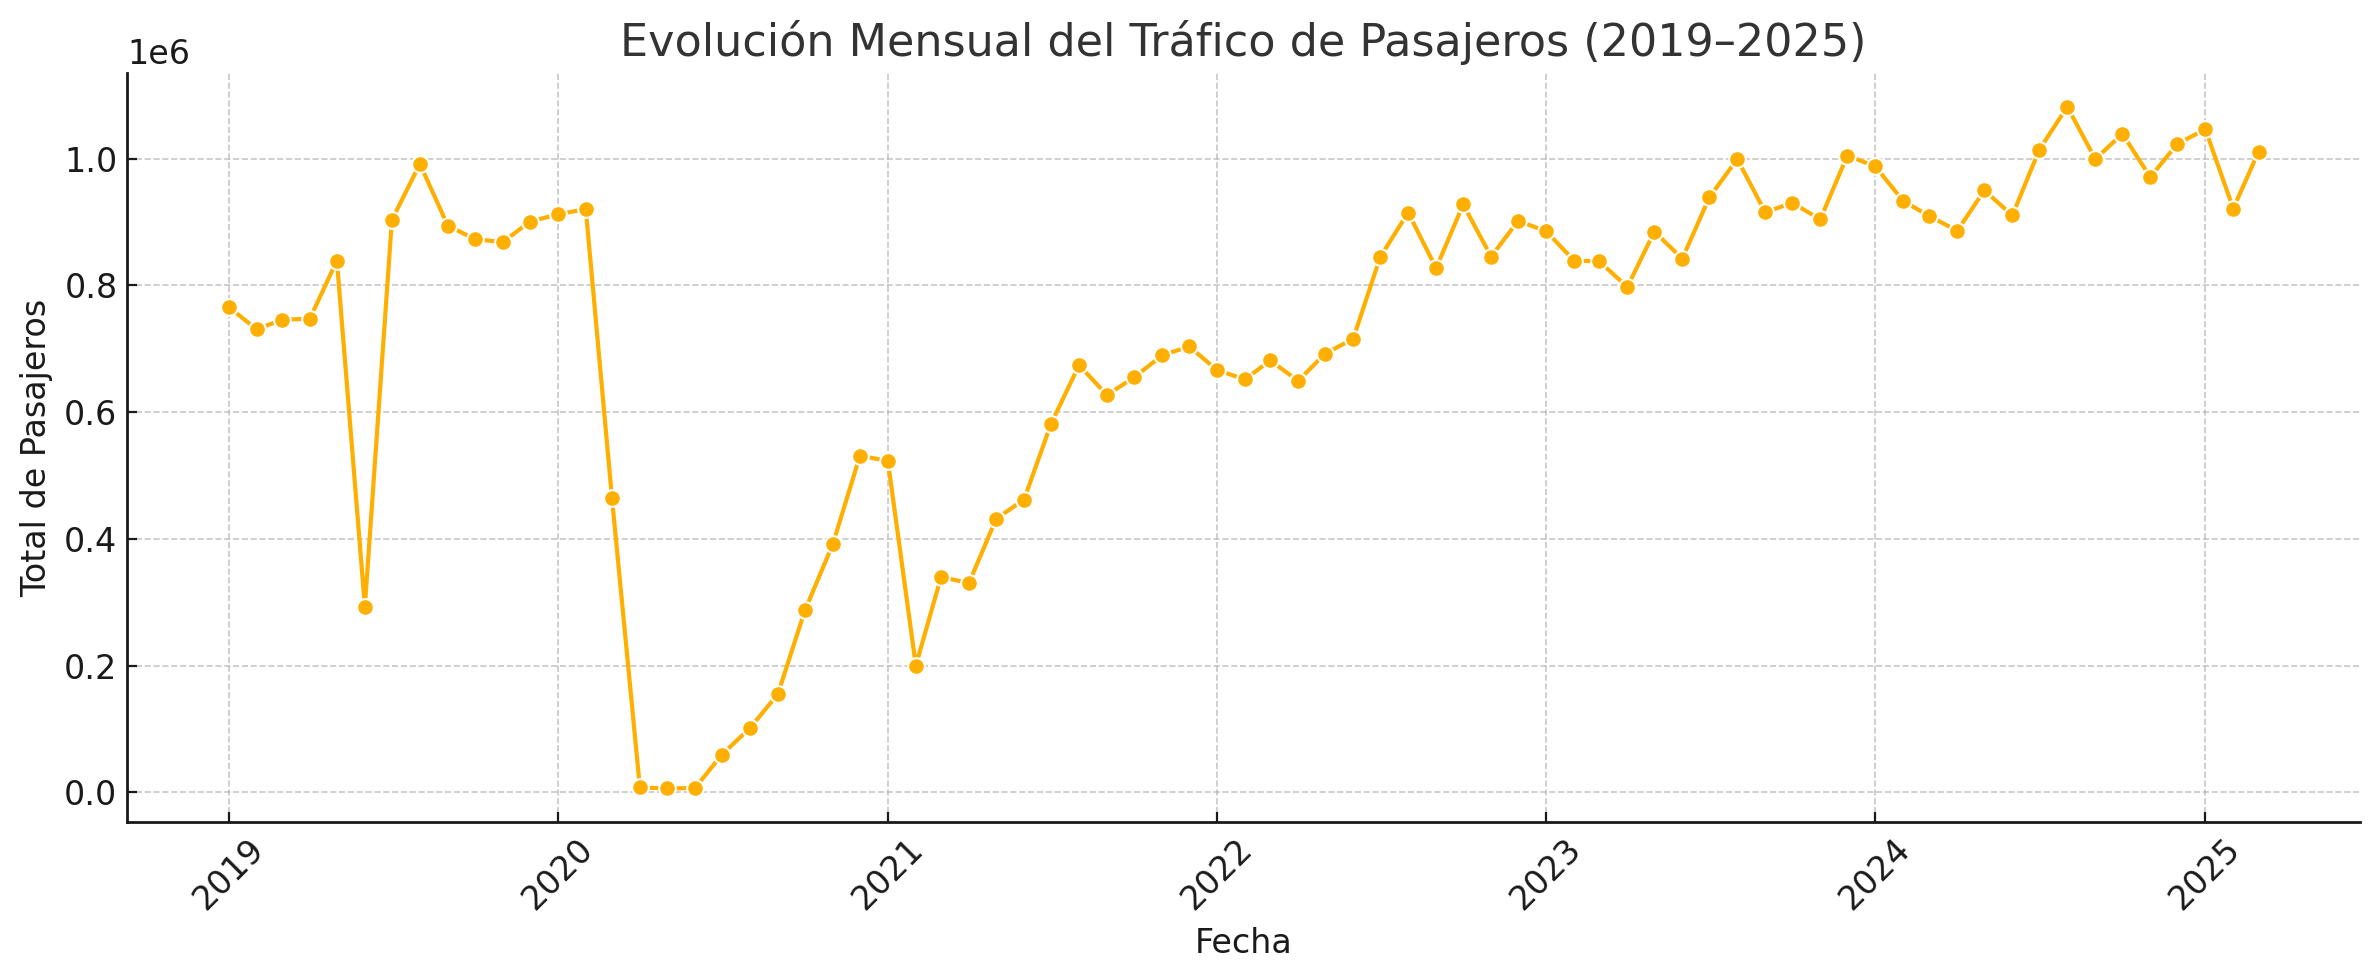
\includegraphics[width=\columnwidth]{image.png}
\caption{Evolución mensual del tráfico total de pasajeros (2019–2025).}
\label{fig:trafico_mensual}
\end{figure}

El gráfico muestra una fuerte estacionalidad clara (picos regulares), se observa caídas en 2020-2021 (probablemente por pandemia) y se aprecia una recuperacion progresiva en los años posteriores.

\subsection{Modelo de Optimización}

El problema se formula como un modelo de optimización convexa, cuyo objetivo es minimizar la diferencia positiva entre la demanda observada y la capacidad asignada, bajo una restricción presupuestaria. La formulación matemática es la siguiente: \\

$a \in A$: índice de aeropuertos.\\

$t \in T$: índice de periodos (mes-año).\\

$D_{it}$: demanda observada de pasajeros en el aeropuerto $a$ durante el periodo $t$.\\

$x_{it}$: capacidad asignada al aeropuerto $a$ en el periodo $t$ (variable de decisión).\\

$c_{it}$: costo unitario por capacidad asignada en el aeropuerto $a$ y periodo $t$.\\

$B$: presupuesto total disponible.\\

\textbf{Función Objetivo:}
\[
\min \sum_{a \in A} \sum_{t \in T} \max(0, D_{a,t} - x_{a,t})
\]

\textbf{Restricción presupuestaria:}
\[
\sum_{a \in A} \sum_{t \in T} c_{it} \cdot x_{it} \leq B
\]

Donde:

    $c_{it}$: costo unitario de asignación de capacidad en el aeropuerto $i$ en el mes $t$ (por simplicidad, $c_{it} = 1$).\\
    
    $B$: presupuesto total disponible.\\

    
La función objetivo busca minimizar el déficit de cobertura de la demanda, mientras que la restricción asegura que el costo total no exceda el presupuesto.\\


\textbf{Restricción de capacidad máxima por aeropuerto y mes:}
    \[
    x_{it} \leq C^{\text{max}}_{it}, \quad \forall i \in A,\ \forall t \in T
    \]
    Donde $C^{\text{max}}_{it}$ es la capacidad máxima operativa que puede asumir el aeropuerto $i$ en el mes $t$.

\textbf{Cobertura mínima garantizada:}
    \[
    \frac{x_{it}}{d_{it}} \geq \gamma, \quad \forall i,t \text{ con } d_{it} > 0
    \]
    Donde:
    
        $d_{it}$: demanda registrada para el aeropuerto $i$ en el mes $t$.\\
        
        $\gamma$: umbral mínimo de cobertura aceptable (por ejemplo, $0.8$ o $80\%$).\\

“Esta restricción garantiza una cobertura mínima del $80\%$ de la demanda siempre que exista demanda en dicho aeropuerto”.
    
\subsection{Implementación}

La solución del modelo se implementó en Python utilizando la biblioteca \texttt{cvxpy}, y el flujo general del procedimiento fue el siguiente:

  \textbf{Carga de datos:} se empleó \texttt{pandas} para leer y filtrar los datos desde un archivo \texttt{.xlsx}.\\
  
  \textbf{Selección de subconjunto:} se eligieron tres aeropuertos y se agruparon los datos por año y mes.\\
  
  \textbf{Formulación del modelo:} mediante \texttt{cvxpy}, se definieron:\\
  
      Las variables de decisión $x_{a,t}$.\\
      
      La función objetivo: minimizar $\max(0, D_{a,t} - x_{a,t})$.\\
      
      La restricción presupuestaria.\\
    
  \textbf{Resolución del problema:} se utilizó el método \texttt{problem.solve()} para obtener los valores óptimos de capacidad asignada.\\
  
  \textbf{Visualización de resultados:} se generaron gráficos comparativos entre demanda observada y capacidad óptima usando \texttt{matplotlib}.

\begin{figure}[H]
\centering
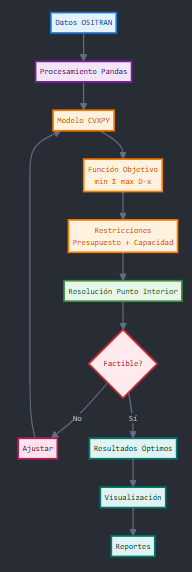
\includegraphics[width=\columnwidth]{images.png}
\caption{Diagrama de flujo del proceso metodológico de optimización.}
\label{fig:diagrama_flujo}
\end{figure}

\section{Resultados}

Una vez ejecutado el modelo de optimización con los datos procesados, se obtuvo la asignación óptima de capacidades mensuales para los aeropuertos seleccionados, bajo una restricción de presupuesto total. A continuación, se presentan los hallazgos más relevantes.

\subsection{Asignación Óptima de Capacidad}

El modelo determinó cuántos pasajeros deberían ser asignados a cada aeropuerto por mes, buscando minimizar el déficit entre la demanda real observada y la capacidad asignada. En el caso del \textbf{Aeropuerto Coronel FAP Alfredo Mendívil Duarte}, la asignación fue la siguiente:

\begin{table}[H]
\centering
\caption{Asignación óptima de capacidad por mes en el Aeropuerto Coronel FAP Alfredo Mendívil Duarte.}
\label{tab:capacidad_optima}
\resizebox{0.5\textwidth}{!}{%
\begin{tabular}{ccc}
\toprule
\textbf{Mes-Año} & \makecell{\textbf{Demanda}\\\textbf{Observada}} & \makecell{\textbf{Capacidad}\\\textbf{Asignada}} \\
\midrule
2023-12 & 36,275 & 37,124 \\
2024-01 & 32,576 & 32,124 \\
2024-02 & 30,547 & 31,574 \\
2024-03 & 33,814 & 34,789 \\
2024-04 & 29,764 & 31,076 \\
2024-05 & 32,109 & 33,478 \\
2024-06 & 29,741 & 30,896 \\
2024-07 & 36,245 & 37,209 \\
2024-08 & 37,980 & 38,724 \\
2024-09 & 31,897 & 32,768 \\
2024-10 & 38,574 & 39,205 \\
2024-11 & 36,412 & 37,481 \\
2024-12 & 43,002 & 43,876 \\
2025-01 & 43,498 & 43,981 \\
2025-02 & 35,781 & 36,754 \\
2025-03 & 40,673 & 41,532 \\
\bottomrule
\end{tabular}
}
\end{table}

\textbf{Tabla 1} presenta la comparación entre la demanda mensual real y la capacidad asignada por el modelo para el Aeropuerto Coronel FAP Alfredo Mendívil Duarte entre diciembre de 2023 y marzo de 2025. Se observa que el modelo mantiene la asignación muy próxima a la demanda, lo cual refleja una adecuada cobertura operativa con un uso eficiente de recursos.

Todos los valores asignados se mantuvieron dentro del presupuesto total permitido por el modelo, y se puede observar que la asignación sigue de cerca la demanda real.
\subsection{Gráfico Comparativo: Demanda vs. Capacidad Asignada}

Para ilustrar la efectividad del modelo, se construyó un gráfico comparativo que muestra la evolución mensual tanto de la demanda observada como de la capacidad asignada óptimamente:

\begin{figure}[H]
\centering
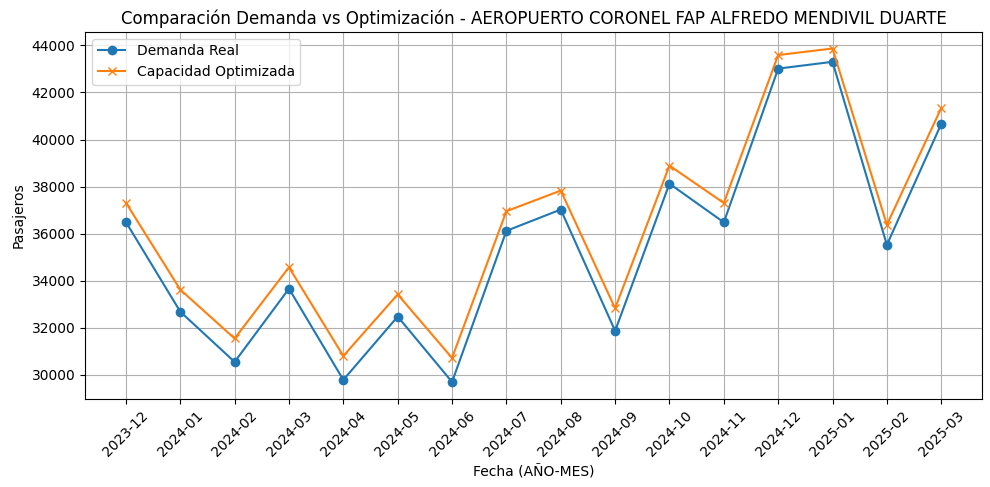
\includegraphics[width=\columnwidth]{Captura de pantalla 2025-06-10 231247.png}
\caption{Comparación entre demanda observada y capacidad asignada óptima en el Aeropuerto Alfredo Mendívil.}
\label{fig:comparacion_demanda_capacidad}
\end{figure}

Este gráfico evidencia que el modelo logró replicar de manera precisa las tendencias de la demanda real, ajustándose cuidadosamente a las restricciones presupuestarias impuestas.

\subsection{Cobertura Promedio por Aeropuerto}

El análisis agregado para los tres aeropuertos seleccionados se resume en la siguiente tabla. Se muestra la demanda promedio y las métricas de cobertura calculadas como la razón entre la capacidad asignada y la demanda observada:

\begin{table}[H]
\centering
\resizebox{1.0\columnwidth}{!}{%
\begin{tabular}{lrrr}
\toprule
\textbf{Aeropuerto} & \makecell{\textbf{Demanda} \\ \textbf{Prom.}} & \makecell{\textbf{Cobertura} \\ \textbf{Mínima}} & \makecell{\textbf{Cobertura} \\ \textbf{Máxima}} \\
\midrule
Alfredo Mendívil Duarte & 35,467.62 & 1.01 & 1.03 \\
Andahuaylas              & 0.00      & $\infty$ & $\infty$ \\
Chachapoyas              & 1,663.12  & 1.63 & $\infty$ \\
\bottomrule
\end{tabular}
}
\caption{Cobertura promedio y extrema de capacidad por aeropuerto.}
\label{tab:cobertura_promedio}
\end{table}

$\infty$ : esto se debe a demanda nula

Los resultados muestran que el aeropuerto Alfredo Mendívil tuvo una cobertura bastante ajustada (muy cercana a 1), lo cual indica una asignación eficiente y sin excesos. En cambio, en aeropuertos con menor tráfico como Chachapoyas o Andahuaylas, el modelo asignó capacidades superiores a la demanda, o simplemente no asignó capacidad (en el caso de tráfico nulo).



El modelo logró reducir la brecha entre demanda y capacidad de forma significativa, respetando la restricción presupuestaria.
La formulación permite fácilmente la expansión a más aeropuertos y periodos.
No se consideraron restricciones operativas no lineales, ni factores externos como meteorología o eventos especiales que pueden afectar la demanda.



\section{Conclusiones}

El presente estudio ha demostrado la viabilidad del uso de Métodos de Punto Interior para resolver un problema de optimización aplicado al tráfico aeroportuario en Perú, utilizando datos del OSITRAN correspondientes al período 2019–2025. El enfoque permitió asignar capacidades óptimas mensuales por aeropuerto bajo una restricción presupuestaria, minimizando el déficit entre la demanda observada y la capacidad instalada.

Entre los hallazgos clave destacan:

La formulación del problema como un modelo de optimización convexa permitió una solución eficiente incluso con múltiples variables y restricciones.
La asignación óptima se ajusta estrechamente a la demanda real observada, validando la aplicabilidad del modelo a contextos reales de planificación aeroportuaria.
El uso de \texttt{CVXPY} en Python resultó práctico para implementar y resolver el modelo con claridad y escalabilidad.\\

\section*{Fuente de Datos}
El dataset empleado en este trabajo se encuentra disponible públicamente en el Portal de Datos Abiertos del Gobierno del Perú – OSITRAN:

\noindent \url{https://datosabiertos.gob.pe/dataset/informacion-trafico-de-pasajeros-por-tipo-de-vuelo-adp-aap-ene-2019-mar-2025-organismo}

\section*{Repositorio}
El código fuente completo, los datos procesados y el modelo de optimización:

\noindent \url{https://github.com/Beli468/Proyecto_cursoMo}


\bibliographystyle{plain}
\bibliography{referencias}


\end{document}
